
    
    
    Heart valves are complex multi-layered structures that prevent backflow by opening and closing depending on the direction of flow. There are four valves in the heart, consisting of two atrioventricular preventing backflow between the atriums and ventricles, the mitral (MV) and tricuspid valves (TV), and two semilunar preventing backflows from the aorta and to the vena cava, the aortic (AV) and pulmonary valves (PV) (Fig. \ref{fig:heartdiagram}). The coordinated movement of the four heart valves enables them to maintain unidirectional blood flow during the cardiac cycle. When healthy, heart valves are incredibly resilient, opening and closing approximately 3 - 4 billion times throughout an average life-span \cite{sacks_biomechanics_2009}. The pressure changes during the cardiac cycle expose the heart valves to constant changes in forces and hemodynamics. This physiological demand is especially harsh on the mitral and aortic valves, needing to withstand average pressures of 80mmHg for the aortic and 120mmHg for the mitral valve to sustain circulation throughout the rest of the body. The biomechanical properties of heart valves must be able to withstand and function efficiently in this complex mechanical environment. Thus, the heart valve leaflets develop and maintain an intricate, highly organized, and multi-scale connective tissue system that allows them to do so \cite{tao_heart_2012}. 

    
    More than five million people are diagnosed with heart valve disease in the United States (US) each year [5, 7], with approximately 95,000 annual valve replacement surgeries, and 20,000 deaths per year [8]. Although valve disease can occur in any of the four valves, diseases of the 
    

%-------------------	begin FIGURE 	-------------------%
\begin{figure}
\centering
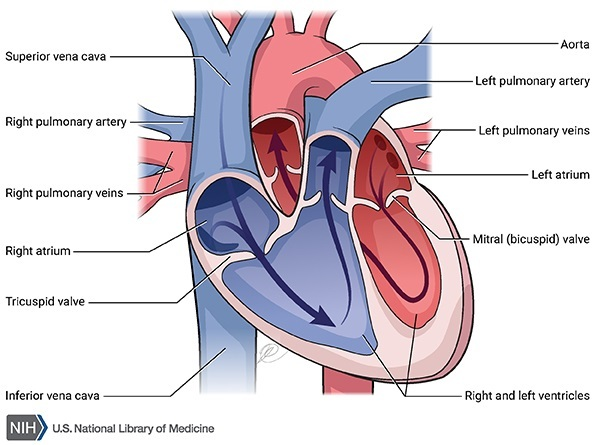
\includegraphics[width=5.0in]{Images/chapter1/heartdiagram.jpeg}
\caption{Artist rendition of the human heart depicting the location of the four heart valves and major vessels (obtained from U.S. National Library of Science website)}
\label{fig:heartdiagram}
\end{figure}
%-------------------	 end FIGURE 	-------------------%

